\clearpage
\section{Shell balance}\label{sec:shell_balance}
En skallbalanse eller ``shell balance'' er en måte å sette opp differensiallikninger som kan brukes til å beskrive hva som skjer i en prosess. Dette gjøres ved å utføre en balanse over en liten bit av system (en ``unit cell''), typisk et lite volum. Herifra antar vi at balansen som gjelder over den lille biten av system også gjelder for hele systemet vi ser på. En slik balanse er basert på balansen vi introduserte i \cref{sec:massetransport}:
\begin{equation}
    \label{eq:gen_balance}
    \text{Akkumulert} = \text{Strøm inn} - \text{Strøm ut} + \text{Generert}
\end{equation}

Når vi setter opp likninger som beskriver det som skjer i en prosess, bruker vi ofte generelle likninger som vi forenkler (eg. Governing equation og Navier Stokes). Dette kan noen ganger være en ganske tungvint måte å gjøre det på, og en shell balance kan da være et godt alternativ for å finne fram til de nødvendige likningene. 

\subsection{Eksempel: Massestrøm gjennom en reaktor med reaksjon}
La oss tenke oss at vi ser på en massestrøm gjennom en reaktor. Vi er da interessert i å se på hvordan systemet endrer seg langs reaktoren. Det første vi kan gjøre er å bestemme oss for en unit cell vi ønsker å gjøre balansen over. I dette tilfellet vil et naturlig valg av en slik unit cell være volumet mellom to tverrsnittsareal i røret. 
\begin{figure}[H]
    \centering
    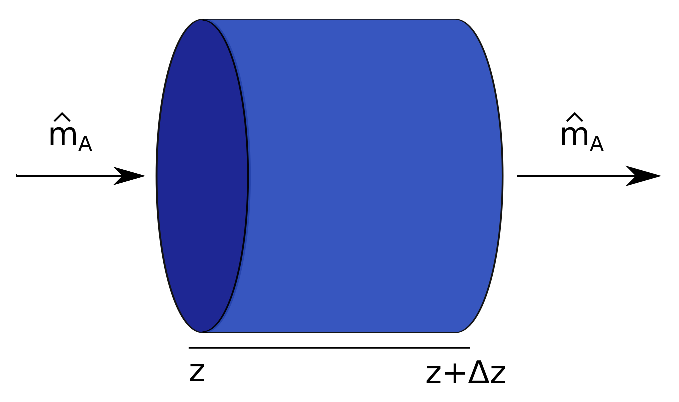
\includegraphics[scale=0.8]{Figures/reactor.eps}
    \caption{Shell balance over et lite volum i en reaktor. A kommer inn i posisjon $z$, reagerer gjennom reaktoren over lengden $\Delta z$ og går ut i posisjon $z+\Delta z$.}
    \label{fig:shell_balance}
\end{figure}

La oss anta at følgende reaksjon skjer gjennom røret: \ce{A ->[\xi_A] B}\\
Videre, la oss sette opp balansen basert på komponent A (merk at vi også kunne satt opp balansen basert på komponent B). Ved å ta i bruk den generelle balansen i \cref{eq:gen_balance} kan en shell balance settes opp på følgende måte:
\begin{equation}
\begin{split}
\label{eq:shellbal}
    \overbrace{\frac{\partial m_A}{\partial t}}^{\text{Akkumulert}} = \overbrace{A \cdot \hat{m}_A\big|_z}^{\text{Inn}} - \overbrace{A \cdot \hat{m}_A\big|_{z+\Delta z}}^{\text{Ut}} - \overbrace{\underbrace{A \cdot \Delta z}_\text{$\Delta V$} \cdot \xi_A}^{\text{Generert}} 
\end{split}
\end{equation}
   Det kan hjelpe å se på benevningnene til utrykkene når du jobber med shell balance for å forstå hvordan du setter opp leddene. Merk at vi $\hat{m}_A$ er fluksen av masse gjennom tverrsnittsarealet i $z$ eller $z + \Delta z$ . For at du ikke skal forvirres av likningen går vi gjennom hvert ledd:
\begin{align*}
     \frac{\partial m_A}{\partial t}:&\, \text{Endring av }m_A\text{ inne i kontrollvolumet}\\
     A \cdot \hat{m}_A\big|_z:&\, \text{ Transport av A inn til kontrollvolumet ved posisjon }z\text{ ganget med tverrsnitt arealet (A)} \\
     A \cdot \hat{m}_A\big|_{z+\Delta z}:&\, m_A \text{ Transport av A ut av kontrollvolumet ved posisjon }z+\Delta z \text{ ganget med tverrsnitt arealet (A)} \\
     A\cdot \Delta z \cdot \xi_A:&\, \text{Tap eller generering av A inne i kontrollvolumet ganget med volumet av unit cellen} 
\end{align*}
Ligningen vi har nå satt har et variaber som er definert i posisjon $z$ og $z + \Delta z$. Som oftest har vi ikke kjennskap til posisjonen $z + \Delta z$ og vi må finne en måte å eliminere $\hat{m}_A\big|_{z+\Delta z}$ fra ligningen vår.
Vi i hovedsak to metoder vi kan benytte oss for å få en løsbar ligning:
\begin{itemize}
    \item Definisjon av den deriverte
    \item Taylorrekke
\end{itemize}
Definisjonen av den deriverte går ut på å hente ut den matematiske definisjonen av derivasjon fra balansen så vi kan substituere differensiallikninger. I dette kompendiet har vi valgt å gå fram med Taylor utvidelse siden vi har alt brukt den i \cref{sec:distributed}. Vi bruker en Taylorrekke på \cref{eq:shellbal} til å approksimere $\hat{m}_A\big|_{z+\Delta z}$. Dette kan gjøres ved å approksimere posisjon $z+\Delta z$ ved bruk av den deriverte i posisjon $z$. Når vi bruker en Taylorrekke til dette, benytter vi oss av samme metode som i \cref{sec:numerisk_approksimasjon} og bruker kun de to første leddene i rekken, til og med den første deriverte:
\begin{equation}
    \label{eq:shell_lin}
    \hat{m}_A\big|_{z+\Delta z} \approx \hat{m}_A\big|_z + \frac{\partial \hat{m}_A}{\partial z}\Big|_z \cdot \Delta z
\end{equation}
Ved å kombinere \cref{eq:shellbal} og \cref{eq:shell_lin} blir balansen enklere å jobbe med siden alle variablene er i posisjon $z$. Notasjonen $\big|_z$ sløyfes herfra for enkelhetens skyld. 
\begin{equation}
    \label{eq:shell_bal_2}
    \frac{\partial m_A}{\partial t} = A \cdot \left(\hat{m}_A - \hat{m}_A - \frac{\partial \hat{m}_A}{\partial z} \cdot \Delta z \right) - \Delta V \cdot r_A
\end{equation}
Her bør det merkes at $\Delta V = A \cdot \Delta z$. Herifra kan vi forenkle likningen, for så og dele på $\Delta V$. Ved å la $\rho_A = m_A/V$ får vi en massebalanse gjennom røret:
\begin{equation}
    \label{eq:final_balance}
    \frac{\partial \rho_A}{\partial t} = \frac{\partial \hat{m}_A}{\partial z} - r_A
\end{equation}
I dette eksemplet burde det merkes at $r_A [=] \frac{kg}{s \cdot m^3}$. For en (litt) mer detaljert forklaring på hvordan vi går fra likning \cref{eq:shell_bal_2} til \cref{eq:final_balance} anbefales det å se ABC-heftet Avsnitt 4.